
\documentclass{article}
\usepackage{graphicx}
\usepackage{amsmath}
\usepackage{float}  % Add float package to control figure placement
\usepackage{listings}
\usepackage{color}


\title{04a Piezo Buzzer Introduction: Making Music with Your Raspberry Pi and GPIO}
\author{Nicholas Bruzzese}
\date{December 06, 2023}

\definecolor{dkgreen}{rgb}{0,0.6,0}
\definecolor{gray}{rgb}{0.5,0.5,0.5}
\definecolor{mauve}{rgb}{0.58,0,0.82}

\lstset{frame=tb,
	language=Python,
	aboveskip=3mm,
	belowskip=3mm,
	showstringspaces=false,
	columns=flexible,
	basicstyle={\small\ttfamily},
	numbers=none,
	numberstyle=\tiny\color{gray},
	keywordstyle=\color{blue},
	commentstyle=\color{dkgreen},
	stringstyle=\color{mauve},
	breaklines=true,
	breakatwhitespace=true,
	tabsize=3
}

\begin{document}
	
	\maketitle
	
	\section*{How Piezo Buzzers Work}
	
	Piezo buzzers are simple devices that convert electrical energy into sound. At the core of a piezo buzzer is the \textbf{piezoelectric effect}, a fascinating phenomenon where certain materials produce an electrical charge in response to mechanical stress, and vice versa. Here's how it works:
	
	\subsection*{The Piezoelectric Effect}
	Piezoelectric materials, such as quartz or certain ceramics, vibrate when an electrical signal is applied to them. These vibrations produce sound waves that we can hear. In a piezo buzzer, a thin piezoelectric element is attached to a diaphragm. When voltage is applied, the element bends and creates sound by vibrating the diaphragm.
	
	\subsection*{Using PWM to Drive a Piezo Buzzer}
	Pulse Width Modulation (PWM) is a technique used to control the signal sent to the piezo buzzer. Instead of providing a continuous voltage, PWM rapidly switches the GPIO pin between HIGH and LOW states. By controlling the frequency of these switches, we can generate sound at specific tones.
	
	\textbf{Summary}
	\begin{itemize}
		\item \textbf{Frequency:} Determines the pitch of the sound. A higher frequency produces a higher-pitched tone.
		\item \textbf{Duty Cycle:} Specifies the proportion of time the signal is HIGH versus LOW. For a piezo buzzer, the duty cycle is typically set to 50\% for consistent tone generation.
	\end{itemize}
	
	On a Raspberry Pi, PWM can be implemented using the \texttt{RPi.GPIO} library or the dedicated \texttt{PWM} hardware channels. In our project, we manually emulate PWM by toggling the GPIO pin at the required frequency, which is sufficient for simple applications.
	
	\section*{Introduction}
	Welcome to the melodious world of Raspberry Pi! Today, we’re going to learn how to make a buzzer sing a tune by controlling GPIO pins. We'll break down the code step by step, explain the logic behind it, and give you a better grasp of physical computing.
	
	\section*{Wiring Diagram}
	This is a simple setup:
	
	\begin{figure}[H]
		\centering
		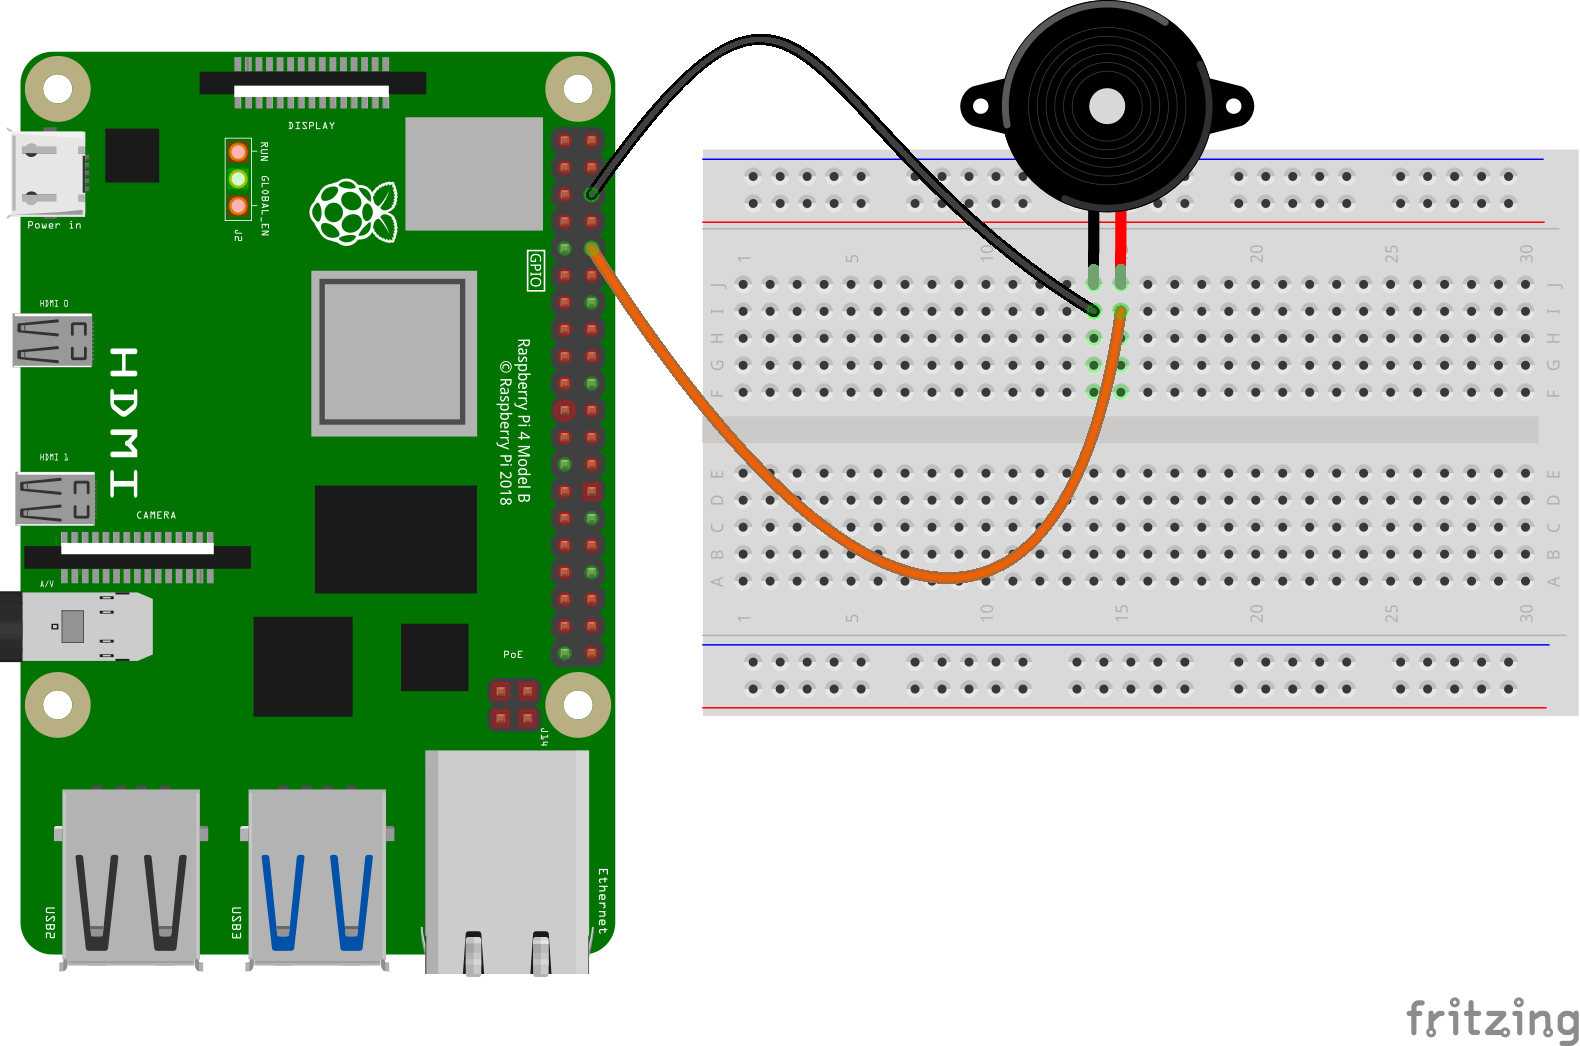
\includegraphics[width=0.8\textwidth]{piezo-buzzer-wiring_bb.png} % Adjust width to 80% of text width
		\caption{Wiring Diagram}
	\end{figure}
	
	\section*{Step 1: Setting the Scene}
	First, we import the necessary libraries. 
	
	\begin{lstlisting}
		import RPi.GPIO as GPIO
		import time
	\end{lstlisting}
	
	\textbf{Explanation:}
	\begin{itemize}
		\item \texttt{RPi.GPIO}: Allows us to control the GPIO pins on the Raspberry Pi.
		\item \texttt{time}: Used for precise timing when controlling the buzzer.
	\end{itemize}
	
	\section*{Step 2: Configuring GPIO}
	\begin{lstlisting}
		GPIO.setmode(GPIO.BCM)
		BUZZER_PIN = 18
		GPIO.setup(BUZZER_PIN, GPIO.OUT)
	\end{lstlisting}
	
	\textbf{Explanation:}
	\begin{itemize}
		\item \texttt{GPIO.setmode(GPIO.BCM)}: Configures GPIO pin numbering to use the Broadcom SoC numbering scheme.
		\item \texttt{BUZZER\_PIN = 18}: This defines the GPIO pin the buzzer is connected to.
		\item \texttt{GPIO.setup(BUZZER\_PIN, GPIO.OUT)}: Sets the pin as an output, allowing us to send signals to the buzzer.
	\end{itemize}
	
	\section*{Step 3: Defining Notes}
	\begin{lstlisting}
		C4 = 261
		G3 = 196
		A3 = 220
		B3 = 247
	\end{lstlisting}
	
	\textbf{Explanation:}
	\begin{itemize}
		\item These constants correspond to musical notes. The number indicates the frequency the buzzer will emit.
	\end{itemize}
	
	\section*{Step 4: Melody and Durations}
	\begin{lstlisting}
		melody = [C4, G3, G3, A3, G3, 0, B3, C4]
		note_durations = [400, 200, 200, 400, 400, 400, 400, 400]
		pause_duration = 300
	\end{lstlisting}
	
	\textbf{Explanation:}
	\begin{itemize}
		\item \texttt{melody}: A list of notes to play. The \texttt{0} represents a pause (no sound).
		\item \texttt{note\_durations}: Specifies how long each note is played in milliseconds.
		\item \texttt{pause\_duration}: Adds a brief silence between notes for better musicality.
	\end{itemize}
	
	\section*{Step 5: Playing Tones}
	\begin{lstlisting}
		def play_tone(pin, frequency, duration):
		period = 1.0 / frequency
		half_period = period / 2.0
		cycles = int(duration / period)
		
		for _ in range(cycles):
		GPIO.output(pin, GPIO.HIGH)
		time.sleep(half_period)
		GPIO.output(pin, GPIO.LOW)
		time.sleep(half_period)
	\end{lstlisting}
	
	\textbf{Explanation:}
	\begin{itemize}
		\item \textbf{Frequency} determines the tone, and \textbf{duration} determines how long it plays.
		\item \texttt{period}: The time for one complete cycle of the waveform.
		\item \texttt{half\_period}: The time for each half of the cycle (on and off).
		\item \texttt{cycles}: The number of cycles the buzzer plays within the duration.
	\end{itemize}
	
	\section*{Step 6: Playing the Melody}
	\begin{lstlisting}
		try:
		while True:
		for i in range(len(melody)):
		note_duration = note_durations[i] / 1000.0
		note_freq = melody[i]
		note_name = note_names.get(note_freq, "Pause")
		
		print(f"Playing {note_name} (Frequency: {note_freq} Hz) for {note_duration} seconds")
		
		play_tone(BUZZER_PIN, note_freq, note_duration)
		time.sleep(pause_duration / 1000.0)
		GPIO.output(BUZZER_PIN, GPIO.LOW)
		except KeyboardInterrupt:
		GPIO.cleanup()
	\end{lstlisting}
	
	\textbf{Explanation:}
	\begin{itemize}
		\item \texttt{try/except}: Allows us to cleanly exit the loop using \texttt{Ctrl+C}.
		\item For each note:
		\begin{itemize}
			\item \texttt{note\_name}: Fetches a human-readable name of the note.
			\item \texttt{play\_tone}: Plays the sound corresponding to the note.
			\item \texttt{GPIO.output(BUZZER\_PIN, GPIO.LOW)}: Ensures the buzzer is turned off after playing.
		\end{itemize}
	\end{itemize}
	
	\section*{Step 7: Cleaning Up}
	When the program exits (via \texttt{Ctrl+C}), we clean up the GPIO settings.
	
	\begin{lstlisting}
		GPIO.cleanup()
	\end{lstlisting}
	
	This step is crucial to prevent the GPIO pins from being left in an unintended state.
	
	
	\newpage
	\section*{Full Code Recap}
	Here is the complete code for reference. It incorporates all the concepts we’ve discussed so far:
	
	\begin{lstlisting}
		import RPi.GPIO as GPIO
		import time
		
		GPIO.setmode(GPIO.BCM)
		BUZZER_PIN = 18
		GPIO.setup(BUZZER_PIN, GPIO.OUT)
		
		C4 = 261
		G3 = 196
		A3 = 220
		B3 = 247
		
		note_names = {C4: "C4", G3: "G3", A3: "A3", B3: "B3"}
		melody = [C4, G3, G3, A3, G3, 0, B3, C4]
		note_durations = [400, 200, 200, 400, 400, 400, 400, 400]
		pause_duration = 300
		
		def play_tone(pin, frequency, duration):
		period = 1.0 / frequency
		half_period = period / 2.0
		cycles = int(duration / period)
		for _ in range(cycles):
		GPIO.output(pin, GPIO.HIGH)
		time.sleep(half_period)
		GPIO.output(pin, GPIO.LOW)
		time.sleep(half_period)
		
		try:
		while True:
		for i in range(len(melody)):
		note_duration = note_durations[i] / 1000.0
		note_freq = melody[i]
		note_name = note_names.get(note_freq, "Pause")
		print(f"Playing {note_name} (Frequency: {note_freq} Hz) for {note_duration} seconds")
		play_tone(BUZZER_PIN, note_freq, note_duration)
		time.sleep(pause_duration / 1000.0)
		GPIO.output(BUZZER_PIN, GPIO.LOW)
		except KeyboardInterrupt:
		GPIO.cleanup()
	\end{lstlisting}
	
	\section*{Experimentation Ideas}
	\begin{itemize}
		\item \textbf{Compose Your Melody}: Replace the \texttt{melody} list with your favorite tune’s notes and durations.
		\item \textbf{Dynamic Pause}: Change \texttt{pause\_duration} to see how it affects the rhythm.
		\item \textbf{Interactive Inputs}: Use buttons or sensors to trigger different melodies!
	\end{itemize}
	
	\begin{itemize}
		\item \textbf{Compose Your Melody}: Replace the \texttt{melody} list with your favorite tune’s notes and durations.
		\item \textbf{Dynamic Pause}: Change \texttt{pause\_duration} to see how it affects the rhythm.
		\item \textbf{Interactive Inputs}: Use buttons or sensors to trigger different melodies!
	\end{itemize}
	
\end{document}